\documentclass[11pt,a4paper]{article}

\usepackage[utf8]{inputenc}
\usepackage[T1]{fontenc}
\usepackage{lmodern}
\usepackage{graphicx}
\usepackage{amsmath}
\usepackage{amssymb}
\usepackage{booktabs}
\usepackage{tikz}
\usetikzlibrary{positioning,arrows.meta}
\usepackage[colorlinks=true,linkcolor=blue!50!black,citecolor=blue!50!black,urlcolor=blue!50!black]{hyperref}
\usepackage{geometry}
\geometry{a4paper, margin=1in}
\usepackage{tocloft}
\setlength{\cftbeforesecskip}{0.35em}
\setlength{\cftbeforetoctitleskip}{0.5em}
\setlength{\cftaftertoctitleskip}{0.5em}

\title{Flea Beetle Damage Assessment:\\A Comparative Study of Classical Computer Vision, Whole-Image, and MIL Approaches}
\author{Emrullah Dagkusu (Matr.-Nr.\ 50268560) \and Federico Rosatelli (Matr.-Nr.\ 50357754)\\[4pt]
  \small Lab Vision Systems (MA-INF 4308), University of Bonn}
\date{30 September 2026}

\begin{document}

\maketitle

\begin{abstract}
Breeding oilseed rape for resistance to the cabbage stem flea beetle requires scoring feeding
damage on thousands of field photographs of young plants (BBCH10--11), a task that is slow and
subjective for human raters. We learn this score from only 470 reliably labelled images and
compare three approaches: classical colour-based computer vision, whole-image regression with a
frozen DINOv3 backbone, and multiple instance learning (MIL), where each plant is scored separately
and the plant scores are pooled into an image score. The whole-image baseline fails (test Spearman
$\rho = -0.11$), because downsampling the photograph removes the damage. Plant-level MIL reaches a
test MAE of 2.4--2.6 percentage points and $\rho$ of 0.76--0.81; fixed pooling rules are at least
as good as learned attention, and adding a pairwise ranking loss gives a small but consistent
improvement (test MAE 2.51, $\rho = 0.78$). On images where the two expert raters disagree, the
model agrees with each rater better than the raters agree with each other. Zero-shot transfer to
two other field trials fails ($\rho = 0.03$ and $0.26$), mainly because of different camera setups
that break frame detection. Classical rules reliably find frames and plants but cannot detect shot
holes; a small RF-DETR hole/pitting detector shows a weak signal after fixing a labelling bug. We
conclude with recommendations for future data recording.
\end{abstract}


\tableofcontents

\section{Introduction}
\label{sec:intro}

The cabbage stem flea beetle (CSFB, \emph{Psylliodes chrysocephala}) is a major pest of oilseed
rape (\emph{Brassica napus}). In autumn, adult beetles feed on the cotyledons and first true
leaves of young plants, leaving small round \emph{shot holes} and shallow yellow/brown
\emph{pitting}. With fewer insecticides available, breeding resistant cultivars is an important
alternative. The Res4StRes project therefore phenotypes hundreds of genotypes in field trials at
six locations. For every plot, three photographs are taken through a $0.1\,\text{m}^2$ metal
frame, and trained raters estimate the percentage of damaged leaf area by comparing the plants
with visual damage scales. Early growth stages (BBCH10--11: cotyledons, possibly the first true
leaf~\cite{bbch}) matter most, because this is when feeding damage threatens crop establishment.

Manual scoring is slow and subjective. Scoring all 8{,}946 images would take a single rater over a
year at 20 minutes per image, and when two universities (JLU and GAU) scored the same 900 images
independently, their scores correlated with only $r = 0.549$. According to the project partners,
the score folds shot holes and pitting into one number and is most likely a per-plant estimate
averaged over the plants in the image. As a result, only 2{,}747 images have scores, and only 470
images, where both raters agree within 5 percentage points, can be regarded as reliable labels.

This makes automatic scoring a \emph{weakly supervised} problem. There is one noisy scalar label
per image, no labels for individual plants or lesions, and very few reliable examples. Moreover,
a seedling covers less than 1\,\% of the image, and a shot hole only a few dozen pixels, so
simply resizing the image for a standard backbone destroys the signal. Finally, the model has to
work on new fields with different soil, lighting and plant age.

We compare three families of approaches on this problem. The first is classical computer vision:
frame detection, colour-based plant segmentation and a direct measurement of damaged pixels, plus
an RF-DETR hole/pitting detector trained on a small annotated set. The second is whole-image
regression with a frozen DINOv3 backbone, the baseline suggested in the project brief. The third
is multiple instance learning (MIL), where each image is a bag of plant regions: a frozen DINOv3
embeds each plant, a shared head scores it, and the plant scores are averaged with weights
proportional to visible plant area. We compare this with uniform pooling and attention-based MIL,
and add a pairwise ranking loss, which was our chosen research direction.

Our contributions are: (i) a leakage-safe benchmark on the 470 reliable images with plot-grouped
splits and a test set that stayed closed during development; (ii) evidence that plant-level MIL
reduces the error of the whole-image baseline by almost half, with area-weighted pooling
outperforming attention pooling; (iii) evidence that adding a ranking loss gives a small but
consistent improvement; (iv) a zero-shot evaluation on two unseen field trials and on images the
two raters disagreed on, which shows where the model fails; and (v) an analysis of which classical
components work, which do not, and why.

Section~\ref{sec:related} reviews related work, Section~\ref{sec:method} describes the methods,
Section~\ref{sec:experiments} presents the results, and Section~\ref{sec:conclusion} concludes with
limitations and recommendations for future data collection.

\section{Related Work}
\label{sec:related}

\paragraph{Classical plant segmentation.} Colour indices such as excess green, together with
thresholds in HSV or CIELAB space, are the standard way to separate vegetation from soil in field
images~\cite{woebbecke1995color,hamuda2016survey}. They are fast and easy to interpret but depend
on lighting and soil colour, and they cannot distinguish lesion types that have similar colours,
such as brown pitting and soil seen through a hole.

\paragraph{Deep learning for plant phenotyping.} Pretrained CNNs and vision transformers are widely
used to classify or regress plant traits from images~\cite{kamilaris2018deep}. Self-supervised
backbones such as DINOv2~\cite{oquab2023dinov2} and DINOv3~\cite{dinov3} provide strong frozen
features, so only a small head has to be trained, which suits small labelled sets. These models
are usually applied at around $224\times224$ pixels, however, which is far too low for
millimetre-sized lesions on seedlings in a full field image.

\paragraph{Multiple instance learning.} In MIL, a label is given for a bag of instances but not
for the instances themselves~\cite{dietterich1997solving,carbonneau2018multiple}. Attention-based
MIL (ABMIL)~\cite{ilse2018attention} learns the pooling weights from the instance features and is
the usual deep MIL baseline, for example for gigapixel pathology slides, which share our problem of
small relevant regions in very large images. Our setting is a regression variant: the bag label is
an average damage over plants, which suggests a fixed weighted mean instead of learned attention.

\paragraph{Learning from comparisons.} When absolute labels are noisy, relative judgements such as
``image A is more damaged than image B'' can be more reliable. Pairwise ranking losses, going back
to RankNet~\cite{burges2005learning}, train a model to order pairs correctly and can be combined
with a regression loss.

\paragraph{Domain shift in agricultural vision.} Models trained on one field, season or set of
lighting conditions often degrade sharply elsewhere. For example, a plant disease classifier with
over 99\,\% accuracy on laboratory images dropped to about 31\,\% on field images~\cite{mohanty2016using},
and multi-site datasets such as the Global Wheat Head Dataset were created to measure
this effect~\cite{david2020global}. We therefore evaluate on unseen trials without any adaptation.

\section{Methodology}
\label{sec:method}

% Pipeline overview, included from chapters/03_methodology.tex
\begin{figure}[tb]
\centering
\resizebox{\textwidth}{!}{%
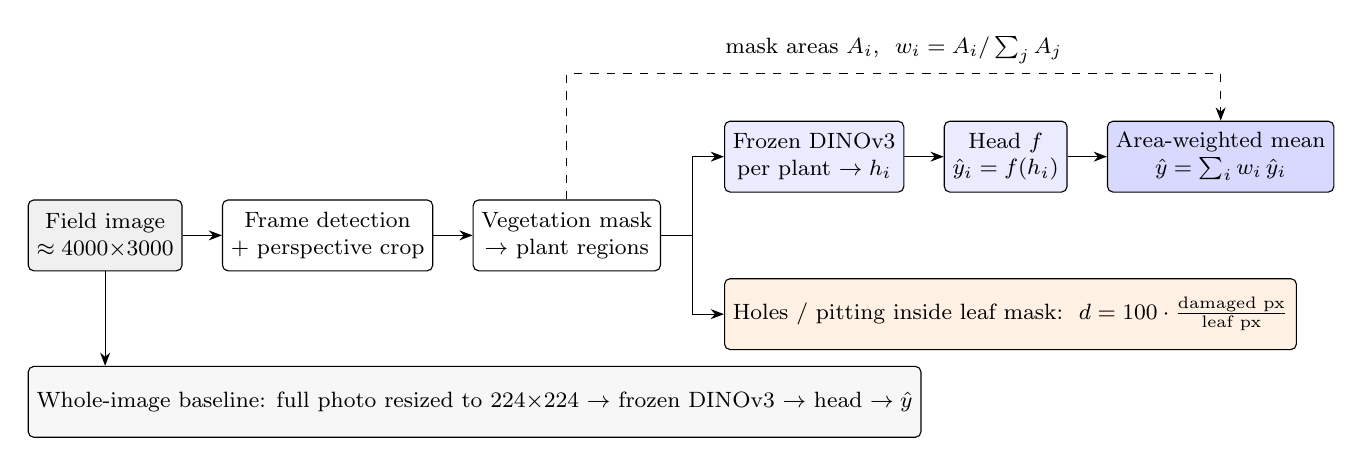
\begin{tikzpicture}[
  font=\footnotesize, >=Stealth, node distance=4mm and 5mm,
  box/.style={draw, rounded corners=2pt, align=center, minimum height=9mm, inner sep=3pt, fill=#1},
  box/.default=white]
  \node[box=gray!12] (img) {Field image\\$\approx 4000{\times}3000$};
  \node[box, right=of img] (frame) {Frame detection\\+ perspective crop};
  \node[box, right=of frame] (veg) {Vegetation mask\\$\to$ plant regions};

  % MIL branch (main)
  \node[box=blue!8, right=8mm of veg, yshift=10mm] (dino) {Frozen DINOv3\\per plant $\to h_i$};
  \node[box=blue!8, right=of dino] (head) {Head $f$\\$\hat y_i = f(h_i)$};
  \node[box=blue!15, right=of head] (pool) {Area-weighted mean\\$\hat y = \sum_i w_i\, \hat y_i$};

  % classical branch
  \node[box=orange!10, right=8mm of veg, yshift=-10mm] (direct)
    {Holes / pitting inside leaf mask:\ \ $d = 100\cdot\frac{\text{damaged px}}{\text{leaf px}}$};

  % whole-image baseline
  \node[box=gray!6, below=12mm of img.south west, anchor=north west] (whole)
    {Whole-image baseline: full photo resized to $224{\times}224$ $\to$ frozen DINOv3 $\to$ head $\to \hat y$};

  \draw[->] (img) -- (frame);
  \draw[->] (frame) -- (veg);
  \draw[->] (veg.east) -- ++(4mm,0) |- (dino.west);
  \draw[->] (veg.east) -- ++(4mm,0) |- (direct.west);
  \draw[->] (dino) -- (head);
  \draw[->] (head) -- (pool);
  \draw[->] (img.south) -- (img.south |- whole.north);
  \draw[->, dashed] (veg.north) |- node[pos=0.75, above]{mask areas $A_i$, \ $w_i = A_i / \sum_j A_j$} ([yshift=6mm]pool.north) -- (pool.north);
\end{tikzpicture}}
\caption{Pipeline overview. Blue: area-weighted MIL (main method), trained with the
image-level expert score only. Orange: classical direct damage measurement. Grey: whole-image
baseline.}
\label{fig:pipeline}
\end{figure}


Figure~\ref{fig:pipeline} summarizes the pipeline. We either (i) regress a score from the whole
downsampled photograph (baseline), or reduce the image to the interior of the metal frame, find the
plant regions, and then (ii) measure damage directly with classical colour rules or (iii) regress a
score for each plant region and pool the plant scores into an image score (MIL). All learned
models share the same frozen DINOv3 backbone and are trained on image-level expert scores only.

\subsection{Data curation and frame extraction}
\label{sec:data}

\paragraph{Calibration set.} We use the 470 BBCH10 images from Gro\ss-Gerau (21.10.2025) for
which the independent JLU and GAU scores differ by less than 5 percentage points. The target is
the damaged share of visible leaf area in percent. The images are split by \emph{plot group} into
331 training, 66 validation and 73 test images, so no plot and no physical image appears in two
splits. The split is stored as a fixed manifest, and every feature cache and checkpoint records the
manifest's SHA-256 hash; training and evaluation refuse to run on a mismatching manifest. An
earlier experiment on a different manifest contained duplicated images across splits; its results
are discarded. The test split stayed closed until model selection was finished.

\paragraph{Frame extraction.} Only plants inside the frame are scored. The galvanized frame bars
are segmented by an HSV colour range on a downscaled image, their outer edges are found with a
probabilistic Hough transform, and the four frame corners are estimated from the clustered lines.
The polygon is inset by 2.5\,\% to remove the bars themselves and rectified with a perspective
warp. Images are read with their EXIF orientation applied, since most field images carry a
non-default orientation tag.

\subsection{Classical computer vision}
\label{sec:classical}

\paragraph{Plant regions and area weights.} Inside the frame, a conservative vegetation mask keeps
pixels with OpenCV hue in $[35,85]$, saturation and value $\geq 40$, and excess
green~\cite{woebbecke1995color} $G-\max(R,B) \geq 5$, followed by morphological opening/closing and
removal of components below 30\,px. Nearby green fragments are merged by a dilation proportional to
the image size (1.8\,\% of the shorter side), so that the cotyledons of one seedling form one
region. Regions with fewer than 150 green pixels are dropped and the remaining boxes are padded by
2.5\,\%. If no frame is detected, the whole image is used instead of the frame crop. The number of green
mask pixels $A_i$ of region $i$ is its visible area, used as the MIL weight in
Section~\ref{sec:mil}.

\paragraph{Direct damage measurement.} Following the supervisor's suggestion, we also measured
damage directly as
\begin{equation}
  d = 100 \cdot \frac{\#\text{pixels classified as hole or pitting}}{\#\text{estimated leaf pixels}} .
\end{equation}
For each plant region, the leaf mask is filled to a solid leaf outline, and non-green blobs
enclosed by it are treated as damage: dark blobs as shot holes and bright yellow/brown blobs as
pitting. A second hole rule additionally accepts enclosed blobs whose CIELAB colour is close to
the surrounding soil, since a real hole shows the soil below. Both rules
were judged by manual review (Section~\ref{sec:res-classical}).

\paragraph{Learned hole/pitting detector.} As the colour rules could not separate holes from
pitting and soil, we annotated bounding boxes for \texttt{shot\_hole} and \texttt{pitting} on 40
training/validation images (342 boxes, SAM-assisted in AnyLabeling) and fine-tuned RF-DETR
Nano~\cite{rfdetr}. Because a typical mark is about $18\times18$\,px in a $4000\times3000$ image, we
train on $640\times640$ tiles around the annotations (71 training / 16 validation tiles). This
detector is exploratory and not used by the scoring models.

\subsection{Whole-image baseline}
\label{sec:baseline}

The baseline follows the project brief: the complete field photograph, without frame cropping,
is resized to $224\times224$ and passed through a frozen DINOv3 ViT-S/16~\cite{dinov3}. Its 384-dimensional \texttt{[CLS]}
embedding goes to a regression head
$\text{Linear}(384,256)\!\to\!\text{ReLU}\!\to\!\text{Dropout}(0.3)\!\to\!\text{Linear}(256,1)$
with a sigmoid scaled to $[0,100]$\,\%. At this resolution a seedling covers only a few pixels,
which motivates the plant-level approach below. The baseline is trained with the Huber loss
and a single seed (42).

\subsection{Multiple instance learning with area-weighted pooling}
\label{sec:mil}

We treat an image as a bag of plant regions (instances) with a single bag label $y$, the expert
score. Plants have no labels of their own, and we do not copy $y$ onto each plant. Every region is
resized to $224\times224$ and embedded with the same frozen DINOv3 backbone, giving features
$h_i \in \mathbb{R}^{384}$. Since the backbone is frozen, all bags are embedded once and cached.
The head $f$ from Section~\ref{sec:baseline} predicts a damage score $\hat y_i = f(h_i)$ for each
plant, and the image prediction is the visible-area-weighted mean
\begin{equation}
  \hat y = \sum_i w_i\, \hat y_i, \qquad w_i = \frac{A_i}{\sum_j A_j},
  \label{eq:weighted}
\end{equation}
as suggested by the supervisor, since the expert estimates the damaged share of the visible leaf
area. Large plants therefore count more, and small false-positive regions have little influence.

We compare this rule with three alternatives. \emph{Uniform} pooling sets $w_i = 1/N$.
\emph{ABMIL}~\cite{ilse2018attention} learns the weights from the features,
$a_i = \operatorname{softmax}_i\!\big(w^\top \tanh(V h_i)\big)$, and regresses from the pooled
feature $\sum_i a_i h_i$. \emph{Gated ABMIL} multiplies the $\tanh$ branch by a sigmoid gate
$\sigma(U h_i)$. The attention width is 128.

All MIL models are trained with the Huber loss, AdamW (learning rate $10^{-3}$, weight decay
$10^{-4}$), batch size 32, and at most 50 epochs with early stopping on validation MAE (patience
10). Each aggregation method is trained with seeds 42, 43 and 44.

\paragraph{Ranking-based training.} The expert scores are subjective, but the \emph{order} of two
images is often clear even when the exact values are not. Following the ranking direction of the
project brief, we train the area-weighted model on pairs $(A,B)$: every training image $A$ is paired
with a random partner $B$ whose score differs by at least $m$, and the loss is
\begin{equation}
  \mathcal{L} = \tfrac12\big[\ell_\delta(\hat y_A, y_A) + \ell_\delta(\hat y_B, y_B)\big]
  + \lambda \max\!\big(0,\, -s\,(\hat y_A - \hat y_B) + m\big),
  \qquad s = \operatorname{sign}(y_A - y_B),
\end{equation}
where $\ell_\delta$ is the Huber loss ($\delta = 1$), $m = 5$ percentage points and
$\lambda = 0.5$. Backbone, pooling and head are identical to the regression model, so only the
training objective differs.

\subsection{Out-of-distribution evaluation}
\label{sec:ood-method}

To test generalization, we apply all trained models zero-shot, without any fine-tuning or
recalibration, to three sets that were never used in development: (i) the field trial Weilburger Grenze
(JLU WG1, 07.10.2025, BBCH10, 906 scored images); (ii) the field trial DSV Asendorf (Trial~1,
15.--17.09.2025, BBCH11, 897 images); and (iii) the 218 Gro\ss-Gerau images from plots outside the
training and validation splits on which JLU and GAU disagreed by more than 5 points. The last set
shares field, date and camera with the training data but has noisy labels, and it lets us compare
model--rater agreement with rater--rater agreement. The pipeline is run unchanged, and we record
whether the frame was found and how many plant regions were extracted in each image.

\subsection{Metrics}
\label{sec:metrics}

We report MAE and RMSE in percentage points, Pearson $r$ and Spearman $\rho$. Because breeders
mainly need to \emph{rank} plots, we also report pairwise ranking accuracy: the fraction of image
pairs whose true scores differ by at least 5 points and whose predicted order is correct. For the
test set we give a bootstrap 95\,\% confidence interval of $\rho$ (5{,}000 resamples). Constant
mean and median predictors serve as reference points.

\section{Experiments and Results}
\label{sec:experiments}

\subsection{Setup}
\label{sec:setup}

All learned models are trained on the 331 training images, selected on the 66 validation images,
and evaluated once on the 73 test images (Section~\ref{sec:data}). Hyperparameters are identical
for all MIL variants (Section~\ref{sec:mil}); every MIL result is the mean $\pm$ standard deviation
over seeds 42, 43 and 44. As references, predicting the training mean (7.38\,\%) or median
(5.0\,\%) for every image gives a validation MAE of 5.45 / 5.41 and a test MAE of 4.45 / 4.01.
A model has to beat these numbers to be useful.

\subsection{Classical computer vision}
\label{sec:res-classical}

Each classical component was checked by manual review of stratified training/validation samples
(never test images) with overlays of every detection. Table~\ref{tab:classical} summarizes the
outcome, and Figure~\ref{fig:qualitative} shows examples.

\begin{table}[tb]
\centering
\small
\caption{Manual audits of the classical components (training/validation images only).}
\label{tab:classical}
\begin{tabular}{@{}llll@{}}
\toprule
Component & Sample & Result & Decision \\
\midrule
Frame detection + crop            & 30 images  & 30/30 approved             & used \\
Plant-region proposal             & 30 images  & 30/30 approved (191 regions)  & used \\
Plant-mask area weights $A_i$     & 40 images  & 40/40 usable               & used \\
Direct damage: leaf mask, pitting & 40 images  & 40/40 acceptable           & exploratory \\
Direct damage: shot holes         & 40 images  & 0/40 usable                & rejected \\
Soil-aware hole rule (CIELAB)     & 20 images  & inconsistent across soils  & rejected \\
Leaf/cotyledon counting           & 8 patches  & systematic over-counting   & rejected \\
RF-DETR hole/pitting detector     & 8 val.\ images & mAP@50 3.5\,\%         & exploratory \\
\bottomrule
\end{tabular}
\end{table}

\paragraph{Frame and plant regions work.} The frame was found in all audited images, and the plant
masks were judged a good approximation of visible leaf area in all 40 images, so they are safe to
use as MIL weights. The green mask does, however, miss strongly discoloured tissue.

\paragraph{Direct damage measurement fails on holes.} Against the expert score, the direct damage
percentage reaches Spearman $\rho = 0.64$ (Pearson $r = 0.46$, $n=40$), but this comes almost
entirely from pitting: the pitting share alone gives $\rho = 0.63$, the hole share only $0.20$.
In manual review the hole detections were unusable in all 40 images, because dark soil seen
through a hole, dark soil next to the leaf and brown pitting have nearly the same colour. The
soil-aware rule did not resolve this. The measurement also underestimates damage by more than an
order of magnitude (mean 0.55\,\% vs.\ 10.2\,\% expert score), mostly because eaten leaf edges
cannot be measured from the remaining leaf shape (Figure~\ref{fig:qualitative}b).

\paragraph{Leaf counting fails because of the damage.} A convexity-defect lobe counter split a
single damaged cotyledon pair into three or four ``leaves'': a feeding notch at the leaf edge is
geometrically indistinguishable from the notch between two leaves. The damage we want to measure
thus breaks the feature, most of all at BBCH10.

\paragraph{RF-DETR: a pipeline bug, then a weak signal.} The first detector reached only
0.4\,\% mAP@50, which we initially attributed to too little data. Plotting the tiled ground truth
revealed the real cause: the tiling script loaded images with automatic EXIF rotation (36 of the 40
images are rotated by 180$^\circ$), while the box coordinates referred to the unrotated image, so
almost every box pointed at soil. After the fix, mAP@50 rose to 3.5\,\% (peak 10\,\% during
training), and predictions now lie on real leaf damage (Figure~\ref{fig:qualitative}c). With only
283 training boxes on $\sim$18\,px objects, and only 61 for pitting, the detector remains far from
usable; we estimate that 150--300 annotated images per class would be needed. The general lesson is
to check a negative result for pipeline bugs before blaming the amount of data.

\begin{figure}[tb]
\centering
\setlength{\fboxsep}{0pt}%
\begin{minipage}[b]{0.235\textwidth}\centering
  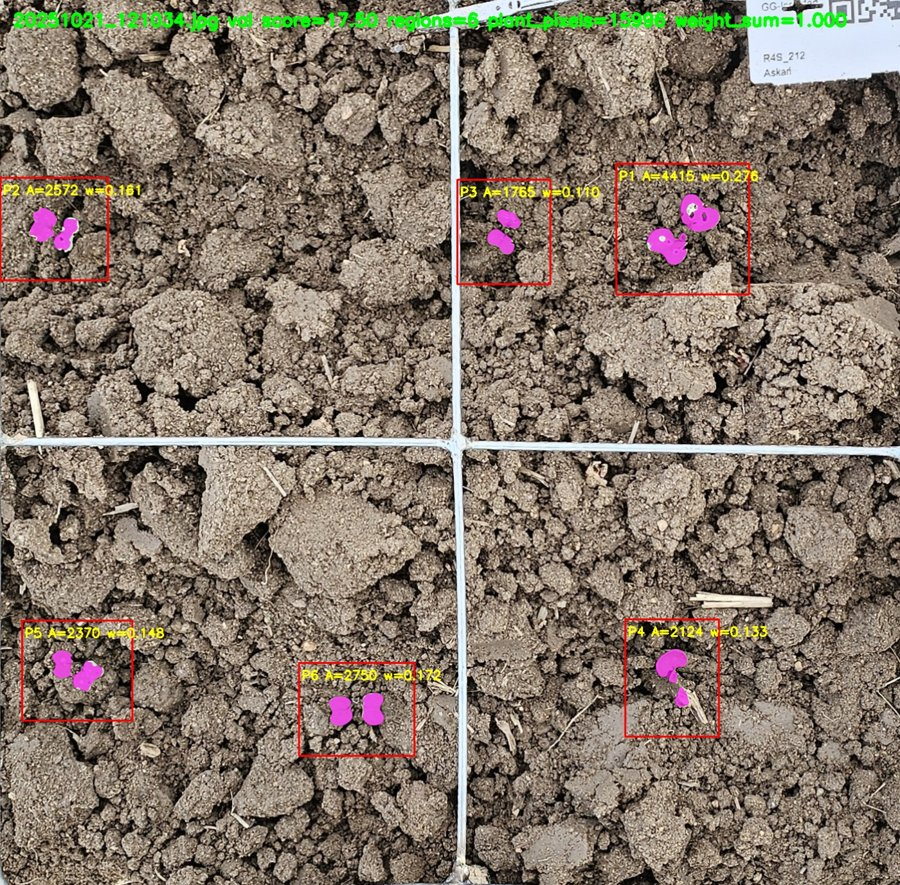
\includegraphics[width=\linewidth]{figures/plant_weights_example.jpg}\\[-1pt]{\small (a)}
\end{minipage}\hfill
\begin{minipage}[b]{0.235\textwidth}\centering
  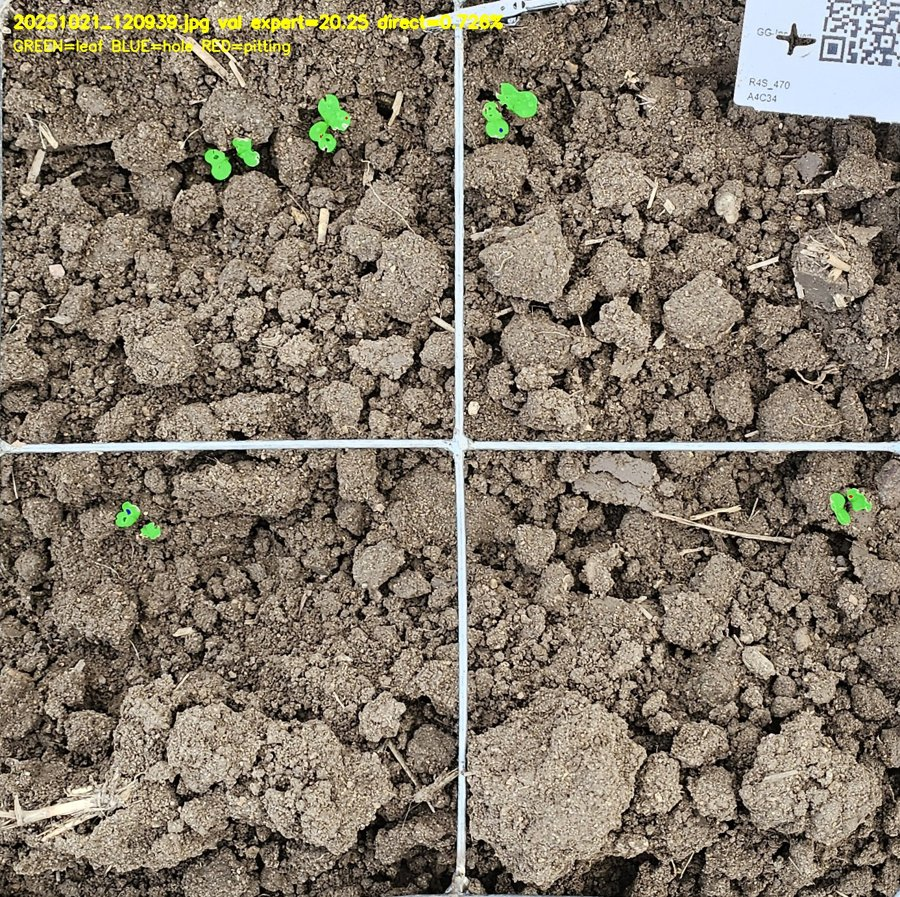
\includegraphics[width=\linewidth]{figures/direct_damage_example.jpg}\\[-1pt]{\small (b)}
\end{minipage}\hfill
\begin{minipage}[b]{0.49\textwidth}\centering
  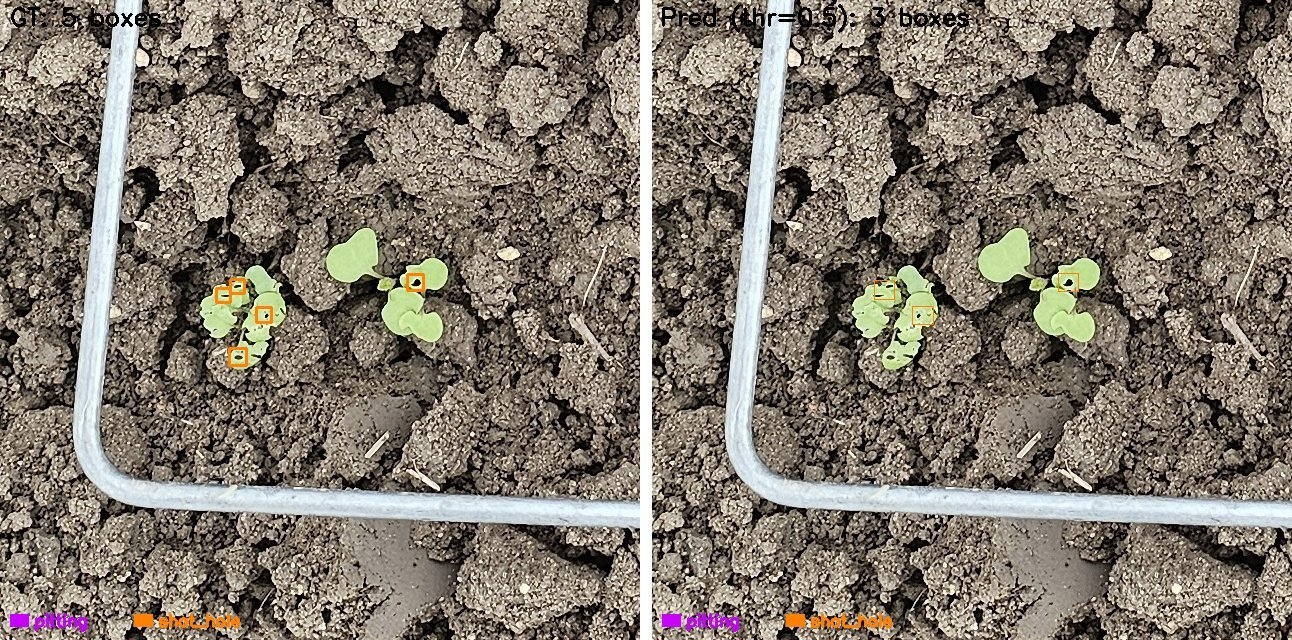
\includegraphics[width=\linewidth]{figures/rfdetr_example.jpg}\\[-1pt]{\small (c)}
\end{minipage}
\caption{(a) Plant regions inside the frame with visible area $A_i$ and weight $w_i$ (expert score
17.5\,\%). (b) Direct damage measurement on an image the experts rated 20.25\,\%: leaf mask in green,
almost no hole or pitting pixels found (0.73\,\%). (c) RF-DETR on a validation tile after the
EXIF fix; left: 5 annotated marks, right: 3 predictions on real damage.}
\label{fig:qualitative}
\end{figure}

\subsection{In-domain scoring: baseline versus MIL}
\label{sec:res-main}

Table~\ref{tab:main} compares all learned models on the Gro\ss-Gerau validation and test sets.

\begin{table}[tb]
\centering
\small
\caption{In-domain results (Gro\ss-Gerau, BBCH10). MIL rows: mean $\pm$ SD over 3 seeds. Pairwise:
share of test pairs with a true difference $\geq 5$ points that are ordered correctly.}
\label{tab:main}
\setlength{\tabcolsep}{4pt}
\begin{tabular}{@{}lccccc@{}}
\toprule
 & \multicolumn{2}{c}{Validation ($n=66$)} & \multicolumn{3}{c}{Test ($n=73$)} \\
\cmidrule(lr){2-3}\cmidrule(l){4-6}
Method & MAE & Spearman $\rho$ & MAE & Spearman $\rho$ & Pairwise \\
\midrule
Constant (training median)        & 5.41 & --    & 4.01 & --     & -- \\
Whole image, DINOv3 (1 seed)      & 5.13 & 0.27  & 4.65 & $-0.11$ & 0.46 \\
\midrule
MIL, uniform pooling              & $2.73 \pm 0.04$ & $0.838 \pm 0.006$ & $\mathbf{2.40} \pm 0.01$ & $\mathbf{0.808} \pm 0.004$ & $0.932$ \\
MIL, ABMIL                        & $2.74 \pm 0.03$ & $0.809 \pm 0.011$ & $2.54 \pm 0.04$ & $0.770 \pm 0.005$ & $0.926$ \\
MIL, gated ABMIL                  & $2.78 \pm 0.02$ & $0.805 \pm 0.011$ & $2.55 \pm 0.03$ & $0.765 \pm 0.007$ & $0.924$ \\
MIL, area-weighted                & $2.69 \pm 0.02$ & $0.853 \pm 0.002$ & $2.62 \pm 0.07$ & $0.763 \pm 0.008$ & $0.924$ \\
MIL, area-weighted + ranking loss & $\mathbf{2.66} \pm 0.04$ & $\mathbf{0.859} \pm 0.001$ & $2.51 \pm 0.05$ & $0.781 \pm 0.002$ & $\mathbf{0.933}$ \\
\bottomrule
\end{tabular}
\end{table}

\paragraph{The whole-image baseline does not learn the task.} Its test MAE of 4.65 is worse than
always predicting the median (4.01), its test correlation is slightly negative, and it orders
only 46\,\% of clearly different image pairs correctly, which is chance level. Its predictions
stay in a narrow band around the mean (SD 2.3 vs.\ 5.6 for the test labels). At $224\times224$ a whole
frame of seedlings shrinks to a few pixels per plant (Figure~\ref{fig:qualitative}b), so the
damage is simply not visible to the backbone.

\paragraph{Plant-level MIL solves it.} All MIL variants reduce the error of the constant predictor
by 35--50\,\% and reach test $\rho$ between 0.76 and 0.81, with over 92\,\% of clearly different pairs
ordered correctly. Since the backbone and the head are the same, the gain comes entirely from
looking at the plants at full resolution instead of the downsampled photograph.

\paragraph{Pooling: small differences, and validation and test disagree.} On validation,
area-weighted pooling was best on both metrics and very stable across seeds, so we selected it
before opening the test set, as the supervisor suggested. On the test set, however, uniform pooling
is clearly better (MAE 2.40 vs.\ 2.62, $\rho$ 0.81 vs.\ 0.76), consistently over all seeds, and the
attention variants lie in between. We report this honestly rather than re-selecting on test. One
plausible explanation comes from how the labels were produced: according to the project partners,
the raters most likely score each plant and \emph{average over plants}, which is exactly uniform
pooling. Area weighting encodes a different target, namely the damaged share of the total leaf
area. With 66 validation and 73 test images, the ranking between the pooling rules is not settled;
what is settled is that fixed pooling is at least as good as learned attention here.

\paragraph{Val--test gap.} For the selected area-weighted model, test $\rho = 0.765$ is lower than
validation $\rho = 0.855$, while the MAE is similar (2.60 vs.\ 2.67). The bootstrap 95\,\% interval
of the test $\rho$ is $[0.62, 0.86]$ and contains the validation value, so with 73 images the gap
is consistent with sampling noise. A second model trained independently by another team member
with the same configuration gives almost identical test results (MAE 2.59, $\rho$ 0.764), which
confirms that the pipeline is reproducible.

\subsection{Ranking-based training}
\label{sec:res-ranking}

Adding the pairwise margin ranking loss to the area-weighted model improves every metric on both
validation and test, and does so for each of the three seeds (last row of Table~\ref{tab:main}):
test MAE drops from 2.62 to 2.51 and test $\rho$ rises from 0.763 to 0.781, with a smaller spread
across seeds. The improvement is small compared with the confidence intervals of a single run, so
we see it as a consistent but modest gain. It supports the idea behind this direction: with
subjective labels, knowing which of two images is more damaged carries useful information beyond
the exact scores. The ranking loss can be combined with any pooling rule; we only tested it with
area weighting.

\subsection{Generalization beyond the calibration set}
\label{sec:res-ood}

\begin{table}[tb]
\centering
\small
\caption{Zero-shot generalization of the area-weighted MIL model (mean over 3 seeds; SD of
$\rho$ $\leq 0.011$). ``Frame'': share of images where the frame was detected. ``Plants'': mean
number of plant regions per image.}
\label{tab:ood}
\begin{tabular}{@{}lrcccccc@{}}
\toprule
 & & & & \multicolumn{2}{c}{Area-weighted} & \multicolumn{2}{c}{+ ranking loss} \\
\cmidrule(lr){5-6}\cmidrule(l){7-8}
Dataset & $n$ & Frame & Plants & MAE & $\rho$ & MAE & $\rho$ \\
\midrule
Gro\ss-Gerau test (reference)            & 73  & 100\,\% & 6.0  & 2.62 & 0.763 & 2.51 & 0.781 \\
Gro\ss-Gerau, raters disagree            & 218 & 99\,\%  & 7.3  & 9.24 & 0.596 & 8.76 & 0.606 \\
Weilburger Grenze (BBCH10)               & 906 & 59\,\%  & 14.3 & 4.32 & 0.031 & 4.29 & 0.070 \\
DSV Asendorf, Trial 1 (BBCH11)           & 897 & 0.1\,\% & 24.4 & 7.73 & 0.264 & 8.24 & 0.239 \\
\bottomrule
\end{tabular}
\end{table}

As the supervisor pointed out, the small test set says little about generalization to other
images. We therefore applied the models without any adaptation to three further sets
(Table~\ref{tab:ood}, Figure~\ref{fig:scatter}).

\paragraph{Images the raters disagree on.} The 218 Gro\ss-Gerau images from plots outside the
training and validation splits whose JLU and GAU scores differ by more than 5 points have the same
field, date and camera as the training data, but noisier and much higher labels (mean 20\,\% vs.\
7\,\%). The model ranks them reasonably ($\rho = 0.60$) but underestimates high damage, since it
has hardly seen scores above 20\,\% during training. Remarkably, the model agrees with each
individual rater ($\rho = 0.50$ with JLU, $0.55$ with GAU) far better than the two raters agree
with each other ($\rho = 0.27$, $r = 0.17$) on these images, where JLU scored on average more than twice as high as GAU (27.4\,\% vs.\ 12.8\,\%). Within its own domain, the model is
therefore at least as consistent as a human rater.

\paragraph{New field trials.} On Weilburger Grenze and DSV the model fails. On Weilburger Grenze it
is essentially uncorrelated with the scores and slightly worse than a constant predictor (MAE 4.32
vs.\ 4.10), and its predictions stay flat across the whole score range. On DSV the rank correlation
is weak ($\rho = 0.26$) and the model overestimates damage (mean prediction 11.8\,\% vs.\ 7.1\,\%),
giving a much higher MAE than a constant (7.73 vs.\ 5.22). No pooling variant does substantially
better on these sets (all $\rho \leq 0.07$ on Weilburger Grenze and $\leq 0.27$ on DSV). Averaging
the three images of each plot, as a breeder would, does not help either (plot-level
$\rho = -0.01$ and $0.23$).

\paragraph{Why the transfer fails.} Inspecting the images shows that the main problem is the
\emph{recording setup}, not only the model (Figure~\ref{fig:ood-examples}). At DSV a different
camera was used, the frame fills the whole photo and has rounded corners, and the frame detector
found it in only 1 of 897 images. At Weilburger Grenze the photos were taken from much farther
away, so the frame covers only part of the image and many plants lie outside it; the frame was
found in 59\,\% of the images. When the frame is missed, the pipeline scores every plant in the
photo (14--24 regions instead of about 6), including plants that the raters did not score, and
each plant is smaller in pixels than in training. Brightness mattered only at DSV, where the darkest third of the images has a clearly higher error (MAE 10.2 vs.\ 6.5 for the brightest third). Even on the Weilburger Grenze images with a detected frame, the correlation stays low
($\rho = 0.17$), so the learned representation itself also transfers poorly. Which part is due to
soil and plant appearance and which to different rating habits at each site cannot be separated
with the available labels.

\begin{figure}[tb]
\centering
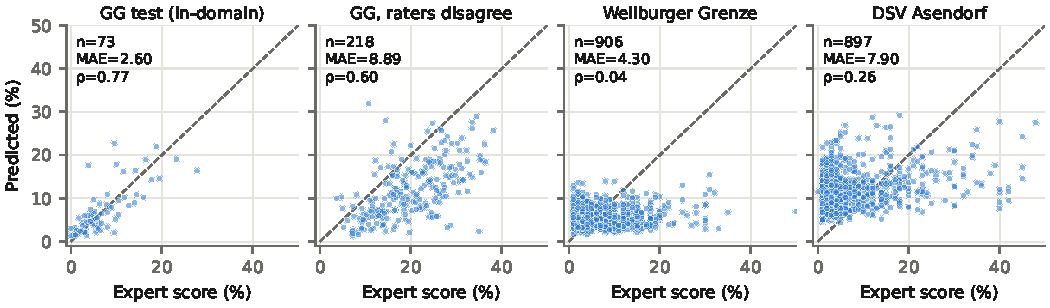
\includegraphics[width=\textwidth]{figures/pred_vs_true.pdf}
\caption{Predicted vs.\ expert score of the area-weighted MIL model (seed 42) on the in-domain test
set and the three generalization sets. Dashed: perfect agreement.}
\label{fig:scatter}
\end{figure}

\begin{figure}[tb]
\centering
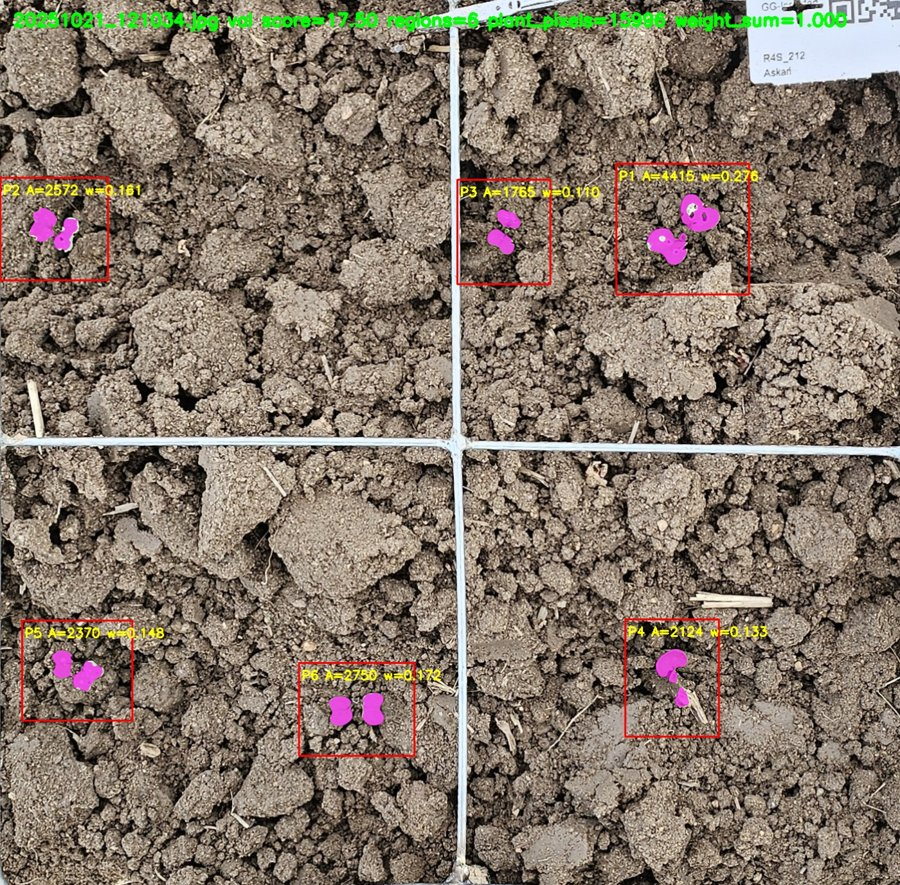
\includegraphics[height=4.2cm]{figures/plant_weights_example.jpg}\hfill
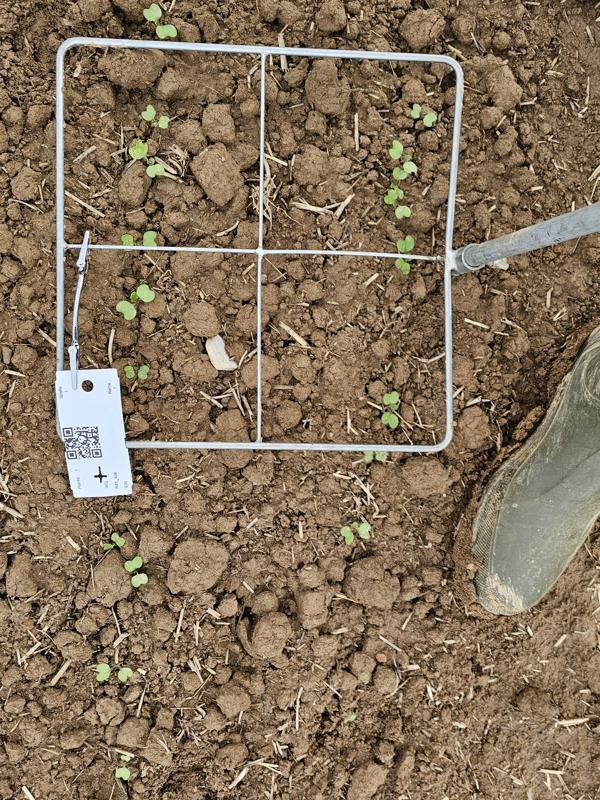
\includegraphics[height=4.2cm]{figures/ood_wg1.jpg}\hfill
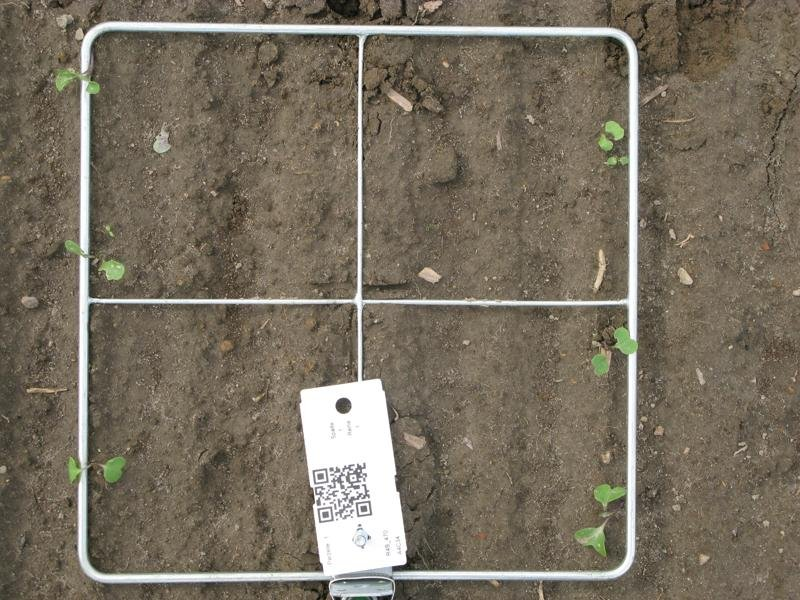
\includegraphics[height=4.2cm]{figures/ood_dsv.jpg}
\caption{Recording setups. Left: Gro\ss-Gerau (training), frame fills the photo, about 6 plants.
Middle: Weilburger Grenze, photo taken from farther away with plants outside the frame. Right: DSV,
different camera and framing; the frame was not detected in 896 of 897 images.}
\label{fig:ood-examples}
\end{figure}

\section{Conclusion and Future Work}
\label{sec:conclusion}

We studied automatic scoring of flea beetle feeding damage on young oilseed rape from field
photographs with very few reliable labels. The three families of approaches behave very
differently.

Classical computer vision is reliable for the geometric steps, i.e.\ finding the frame and the
plants and measuring their visible area, but not for the damage itself: holes, soil and brown
pitting cannot be separated by colour, and eaten leaf edges do not show up in a pixel count. We
therefore see it mainly as preprocessing and as a source of interpretable side features such as
pitting area. Whole-image regression with a frozen DINOv3 fails (test $\rho = -0.11$), because
downsampling a field photograph to $224\times224$ erases the seedlings. Plant-level MIL works
in-domain, with a test MAE of 2.4--2.6 percentage points and $\rho$ of 0.76--0.81. Fixed pooling
rules were at least as good as learned attention. Area weighting won on validation and uniform
pooling on test; given how the raters score, uniform pooling may be closer to the label
definition. Adding a pairwise ranking loss gave a small improvement for all three seeds.
On the Gro\ss-Gerau images where the two raters disagreed, the model agrees with each rater
better than they agree with each other. On new field trials, however, the model does not
generalize ($\rho$ 0.03 and 0.26), mainly because the frame is not found and plants outside the
frame are scored, and partly because the learned features transfer poorly to other fields.

\paragraph{Limitations.} All reliable labels come from one field on one day, so our in-domain
numbers describe a single recording condition. The labels are subjective averages that mix holes
and pitting, which limits the achievable accuracy and makes the choice of pooling rule ambiguous.
Validation and test sets are small (66 and 73 images), so differences below about 0.1 in $\rho$
between methods are uncertain. Only 40 images were annotated for the hole/pitting detector, and
only 7 of the 217 genotypes have more than one plot in the calibration set, so we did not attempt
a genotype resistance ranking.

\paragraph{Recommendations for future data recording.} Most of the generalization failure could be
avoided at recording time:
(i) use the same frame and hold the camera so that the frame fills the photo, at a fixed height,
at every site;
(ii) give the frame a marker that is easy to detect, e.g.\ coloured corners or an ArUco marker next
to the QR code;
(iii) score a small calibration set (50--100 images) with two raters at every site and date, so that
each new domain has some reliable labels;
(iv) record, per image, whether single plants or the image as a whole were scored, and score holes
and pitting separately;
(v) annotate 150--300 images per damage class with boxes or masks to make a lesion detector usable.

\paragraph{Future work.} The next steps are, in order of expected benefit: a more robust frame and
plant detector (e.g.\ SAM-based segmentation of plants, as suggested in the project brief) and
re-running the out-of-distribution evaluation; few-shot calibration of the head with a few
labelled images per new site; domain adaptation by self-supervised pre-training on the 8{,}946
unlabelled images; weak labels from a vision-language model; and combining the ranking loss with
uniform pooling. A learned leaf and lesion segmentation would also allow the plant counts, leaf
counts and hole/pitting statistics requested by the project partners.


\clearpage
\bibliographystyle{plain}
\bibliography{references}

\end{document}
